\chapter{The first experiment}\label{chapter:the-first-experiment}
When we first thought about using the LSP in this project we decided to try it first hand with a simple implementation of the ECLAIR analysis in the IDE. The first iteration consisted of a Language Server which simply listened to file changes which would in turn trigger a new ECLAIR analysis each time using the CLI. Then the analysis output would be parsed, converted to LSP Diagnostics and sent over to the client. 

\begin{figure}[ht]
	\centering
	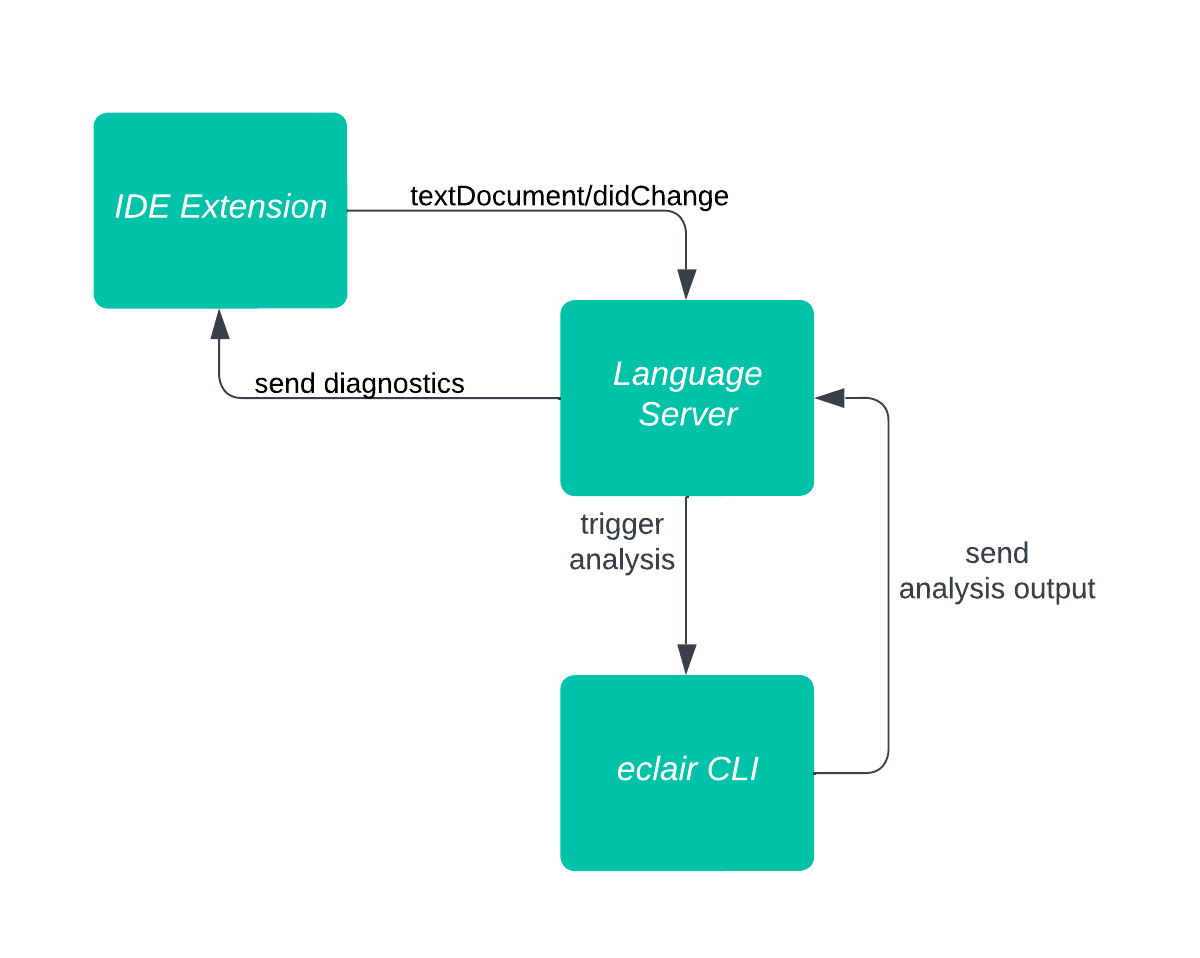
\includegraphics[width=0.9\textwidth]{Immagini/the_first_experiment_flow.jpg}
	\caption{First experiment with the Language Server Protocol}
	\label{fig:one}
\end{figure}

\clearpage

In order to fully understand the benefits the LSP could give us, we realized two extensions, for VSCode and Sublime Text. In both cases we could observe that, with just a few lines, we were able to see the violations marked in the file.

\begin{lstlisting}[caption={First Sublime Text working configuration}, label={lst:block_struct}]
{
  ``clients": {
    ``elcair": {
      ``command": [
        ``eclair-server",
        ``--stdio"
      ],
      ``enabled": true,
      ``languages": [
        {
          ``languageId": ``c"
        }
      ]
    }
  },
  ``log_debug": true
}
\end{lstlisting}

\begin{lstlisting}[caption={First VSCode working extension}, label={lst:block_struct}]
const { LanguageClient } = require(``vscode-languageclient")

module.exports = {
  activate(context) {
    const executable = {
      command: ``eclair-server",
      args: [``--stdio"]
    }

    const serverOptions = {
      run: executable,
      debug: executable
    }

    const clientOptions = {
      documentSelector: [{
        scheme: ``file",
        language: ``c"
      }]
    }

    const client = new LanguageClient(
      ``eclair-extension-id",
      ``Eclair",
      serverOptions,
      clientOptions
    )

    context.subscriptions.push(client.start())
  }
}
\end{lstlisting}